\documentclass[a4paper,12pt]{scrartcl}
\usepackage[margin=2cm,bindingoffset=0cm]{geometry}
\usepackage{ucs}
\usepackage[utf8x]{inputenc}
\usepackage[ngerman]{babel}
\usepackage{fontenc}
%\usepackage[pdftex]{graphicx}
\usepackage{listings}
\usepackage{amssymb}
\usepackage{amsmath}
\usepackage{wasysym}
\usepackage{graphicx}
\usepackage[pdftex]{hyperref}
\author{
Verena Käfer (2551188),\\
Niklas Schnelle (2573250),\\
Peter Vollmer (2553704)}
\date{erstellt am 08.12.2010\\
Version: 1.2}
\title{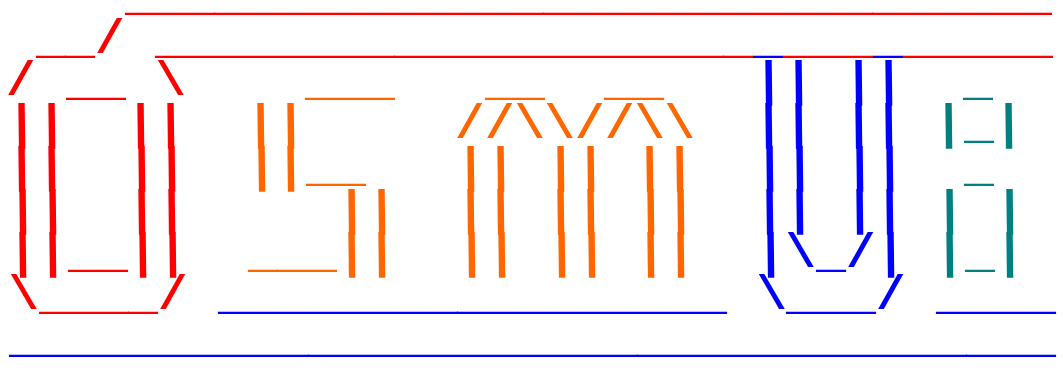
\includegraphics[width=15cm]{../projektplan/Logo_Osmui.png} \\ 
Entwurf von OsmUi}

\begin{document}
\maketitle
\newpage
\tableofcontents
\newpage

\section{Einleitung}
Die folgenden Abschnitte beschreiben den Entwurf und die Architektur von OsmUi.
\subsection{Das Software-System}
OsmUi stellt eine Benutzeroberfläche für das Kommandozeilen-Tool Osmosis dar. Die Implementierung erfolgt in Java 6, die Oberfläche wird mit Swing realisiert. Für die graphische Darstellung der Pipelines wird auf JGraph zurückgegeriffen. Die Pipelines werden entweder in smu-Dateien gespeichert oder als Kommandozeilenscripst exportiert.
\subsection{Entwurfsprinzipien}

\subsection{Überblick über den Entwurf}
In den folgenden Abschnitten werden zuerst die Architektur (Kapitel 2) und dann die einzelnen Komponenten (Kapitel 3) beschrieben. Die genaue Dokumentation der Klassen und Methoden erfolgt direkt im Programm als JavaDoc. Desweiteren soll dieses Dokument, die Entwurfsentscheidungen dokumentieren.

\section{Architektur}
Osmui setzt sich aus mehreren Komponenten zusammen. Diese sollen so organisiert werden, dass der Zusammenhalt innerhalb der Komponenten groß und die Kopplung zwischen ihnen möglichst klein ist. Zur Strukturierung des Systems sollen weiterhin GUI-Komponenten klar von den dahinter liegenden Modellen getrennt werden. Da OsmUi jedoch selbst Oberfläche für ein Kommandozeilenwerkzeug ist, existiert keine klare Frontend/Backend-Trennung.\\
Im folgenden sind die Komponenten beschrieben, wobei jeder Komponente im später System einer Java-Klasse entspricht.

%\subsection{Komponentenübergreifende Funktionen}

\section{Komponenten}
\subsection{Komponente: TaskBox}
Die TaskBox implementiert eine GUI Komponente die alle zum momentan selektierten Task kompatiblen Tasks anzeigt. Ist kein Task selektiert zeigt sie nur die Tasks an, die keine Vorbedingungen haben. Auch kann über sie ein Task zum TaskModel hinzugefügt werden.
\subsubsection{Schnittstelle}
Die TaskBox implementiert das Interface TaskSelectEventListener um auf die Selektion eines Tasks in der PipelineBox zu reagieren. Erstellt wird eine TaskBox unter Angabe des ihr zu Grunde liegenden Modells. Dieses kann über getter/setter auch nachträglich geändert werden.
\begin{center}
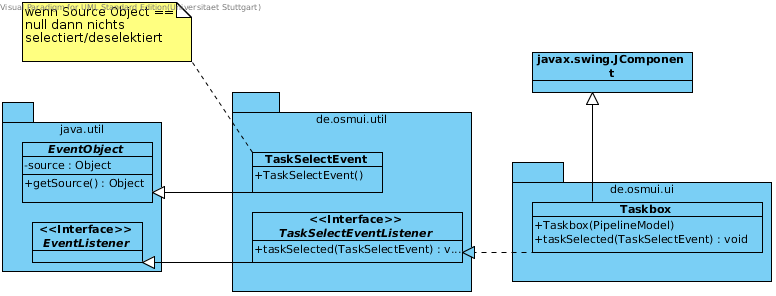
\includegraphics[width=17cm]{Schnittstelle_TaskBox.png}
\end{center}
\subsubsection{Protokoll}
Nach der Konstruktion muss die TaskBox noch als EventListener registriert und zur Benutzeroberfläche hinzugefügt werden.
\subsubsection{Verhalten}
Die Taskbox fügt ausgelöst durch Nutzerinteraktion neue Tasks in das PipelineModel ein.
%\subsubsection{Interne Realisierung}
\subsubsection{Realisierte Anforderungen}
Diese Komponente ermöglicht das Hinzufügen von neuen Tasks.

\subsection{Komponente: PipelineBox}
Die PipelineBox zeigt die aktuelle Pipeline an und ermöglicht dem Benutzer Tasks zu selektieren, zu verschieben und zu löschen. 
\subsubsection{Schnittstelle}
Die PipelineBox interagiert mit anderen Komponenten durch das erzeugen von TaskSelectEvent's und TaskDoubleclickEvent's.
Sie ist dadurch gut vom Rest des Systems getrennt. Dies ist möglich, da sie alle komplexeren Interaktion mit dem Benutzer wie das verschieben von Tasks, löschen von Tasks und verbinden von Tasks intern und unter Benutzung anderer Komponenten regeln kann.
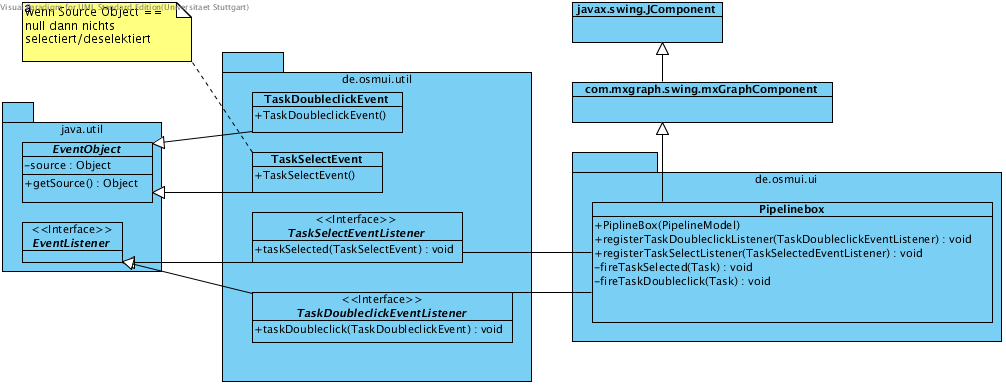
\includegraphics[width=17cm]{Schnittstelle_PipelineBox.png}
\subsubsection{Protokoll}
Wird ein Tasks selektiert, so wird ein TaskSelectEvent ausgelöst. Wird kein Task selektiert, so wird ein TaskSelectEvent mit Source gleich null ausgelöst. Ein Doppelklick auf ein Task löst ein TaskSelectEvent und ein TaskDoubleclickEvent aus.
\subsubsection{Verhalten}
Die PipelineBox regelt die grafische Interaktion des Benutzers mit der Pipeline, wobei das hinzufügen von Tasks wiederum durch die TaskBox realisiert wird.
\subsubsection{Interne Realisierung}
\subsubsection{Realisierte Anforderungen}
Grafische Darstellung der Osmosis Pipeline

\subsection{Komponente: ParameterBox}
Die ParameterBox zeigt die Parameter des aktuell selektierten Tasks an und ermöglicht dem Benutzer diese zu ändern. 
\subsubsection{Schnittstelle}
\begin{center}
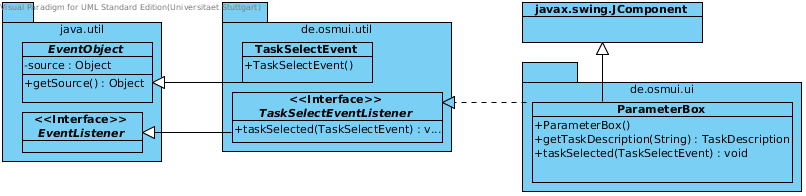
\includegraphics[width=17cm]{Schnittstelle_ParameterBox.png}
\end{center}
\subsubsection{Protokoll}
Um die Boundingbox zu benutzen, muss sie als erstes geöffnet werden (TaskDoubleklickEvent). Dann können die Daten geändert werden. Danach wird sie wieder geschlossen.
\subsubsection{Verhalten}
Die ParameterBox wird über die Auswahl eines Tasks durch taskSelectedEvents informiert und kommt über das EventObject an das eigentliche Task Objekt, in ihm werden die Parameter direkt verändert.
%\subsubsection{Interne Realisierung}
\subsubsection{Realisierte Anforderungen}
Einstellen von Task Parametern

\subsection{Komponente: TaskManager}
Der TaskManager verwaltet die Informationen zu Taskstypen, prüft Kompatibilitäten zwischen Tasks und dient als Factory für Tasks. Diese werden dabei aus den TaskDescription Objekten erzeugt, welche aus einer \glqq osmosis-tasks.xml'' Datei gelesen wurden. Die Spezifikation der TaskDescription Klasse und weiterer hierfür notwenidiger Klassen wird mit Hilfe
der \glqq Java Architecture for XML Binding`` erzeugt.
\subsubsection{Schnittstelle}
Der Zugriff aus TaskDescriptions und das erzeugen von Tasks mit Hilfe des TaskManagers erfolgt durch Angabe des Tasknamens
von der Form \glqq fast-read-xml'' dies ermöglicht ein einfacheres und zugleich erweiterbares Interface, welches nicht von der Realisierung der Task Objekte abhängt.
\begin{center}
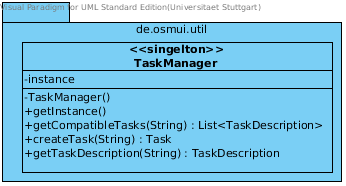
\includegraphics[width=8cm]{Schnittstelle_TaskManager.png}
\end{center}
\subsubsection{Protokoll}
Der Taskmanager bekommt eine Anfrage zu einem Task und gibt dann die passenden Informationen heraus.
\subsubsection{Verhalten}
\subsubsection{Interne Realisierung}
\subsubsection{Realisierte Anforderungen}
Bereitstellen einer abstrahierten Form für Osmosis Tasks die leicht erweiterbar und flexibel ist.

\newpage
\subsection{Komponente: PipelineModel}
Das PipelineModel hält die interne nichtgrafische Repräsentation der Pipeline und bietet Schnittstellen für die Verwaltung von Tasks in der Pipeline und der Validierung einer Pipeline. (Feststellen ob sie ausführbar ist)
\subsubsection{Schnittstelle}
Der Zugriff auf Tasks erfolgt direkt über Referenzen auf konkrete Task Objekte, dies können zum Beispiel erreicht werden
indem die Pipeline von den SourceTasks (also denjenigen ohne eingehende Pipes) durchlaufen wird. Über Task Referenzen können Tasks im PipelineModel verbunden oder gelöscht werden. Desweiteren löst das TaskModel ein ModelChangedEvent aus sobald das Modell verändert wurde. Nur für die Interaktion mit der PipelineBox vorgesehen ist der direkte Zugriff auf die eingebettete mxGraph Komponente.
\begin{center}
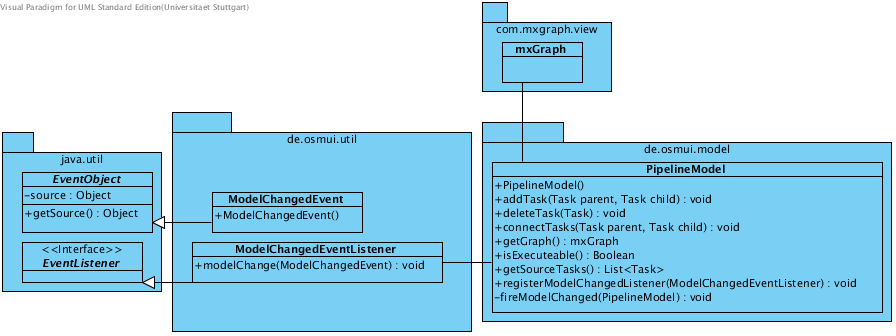
\includegraphics[width=17cm]{Schnittstelle_PipelineModel.png}
\end{center}
\subsubsection{Protokoll}
Die Komponente bekommt Anfragen über das Model und gibt die passenden Informationen zurück.
\subsubsection{Verhalten}
\subsubsection{Interne Realisierung}
Das PipelineModel benutzt zum Speichern der Pipeline eine mxGraph Komponente, hierbei wird jedoch versucht durch entsprechendes Design des PipelineModels sowie der Task Objekte (die eigene Methoden implementieren um von einer Task zu
den angeschlossenen nachbar Tasks zu gelangen und die Kanten (Pipes) zu inspizieren) die Funktionalität des mxGrap Modells
weitestgehend zu Kapseln so, dass dieses gegebenenfalls ersetzt werden kann ohne anderen Code ändern zu müssen.
Dabei ist es wichtig darauf zu achten, die getGraph() Methode nur äußerst sparsam einzusetzen, genauer gesagt nur in der TaskBox Komponente. (Leider ist eine bessere Kapselung wie zum Beispiel mit C++ friend Klassen in Java nicht auf dieser Ebene realisierbar)
\subsubsection{Realisierte Anforderungen}
Modellieren einer Pipeline.

\subsection{Komponente: PipeImEx}
Die Komponente PipeImEx übernimmt die Funktionalität des Importierens und Exportierens. Dabei verwendet sie die PipelineModell Komponente sowie die einzelnen Task/Pipe Objekte zum Traversieren des Pipelinegraphs. Sie verwendet \textbf{nicht} PipelineModel.getGraph()
\subsubsection{Schnittstelle}
\begin{center}
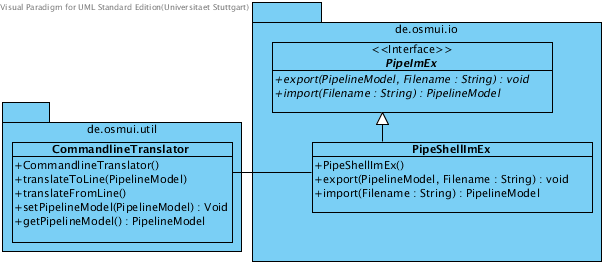
\includegraphics[width=17cm]{Schnittstelle_PipeImEx.png}
\end{center}
\subsubsection{Protokoll}
Importieren: \\
Die Komponente bekommt einen filename und importiert diese Pipeline dann.\\
Exportieren: \\
Die Komponente bekommt einen filename und eine Pipeline. Diese wird dann exporiert.
\subsubsection{Verhalten}
\subsubsection{Interne Realisierung}
Die Komponente nutzt ein allgemeines Interface sowie eine dieses Interface realisierende Klasse, die den eigentlichen Shell Im-/Export übernimmt. Für das eigentliche Erzeugen des Osmosis Aufrufs wird eine Helferklasse Namens CommandlineTranslator verwendet, die es ermöglicht diese mehrfach benötigte relativ komplexe Arbeit zu kapseln.
\subsubsection{Realisierte Anforderungen}
Importieren und Exportieren von Pipelines in Shellscripte.

\subsection{Komponente: Help}
Diese Komponente stellt einen Dialog zum einsehen der Online-Hilfe bereit.
\subsubsection{Schnittstelle}
Der Hilfe Dialog wird erzeugt und arbeitet dann selbstständig.
%\subsubsection{Protokoll}
%\subsubsection{Verhalten}
\subsubsection{Interne Realisierung}
Es wird eventuell eine Library verwendet um die Hilfe anzuzeigen.
\subsubsection{Realisierte Anforderungen}
Bereitstellen einer Online-Hilfe
\subsection{Komponente: BoundingBoxChooser}
Die Komponente BoundingBoxChooser übernimmt die Funktionalität um einen Kartenausschnitt grafisch auszuwählen.
\subsubsection{Schnittstelle}
Die Schnittstelle wird durch die API bereit gestellt.
%subsubsection{Protokoll}
%\subsubsection{Verhalten}
%\subsubsection{Interne Realisierung}
\subsubsection{Realisierte Anforderungen}
Kartenausschnitte grafisch wählen.

\subsection{Komponente: I18N}
Die Komponente I18N übernimmt die Funktionalität der Internationalisierung.
\subsubsection{Schnittstelle}
\begin{center}
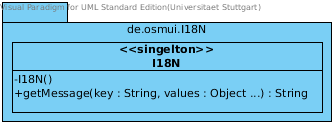
\includegraphics[width=8cm]{Schnittstelle_I18N.png}
\end{center}
\subsubsection{Protokoll}
\subsubsection{Verhalten}
Diese Komponente ermöglicht es zu einem Keystring eine lokalisierte Version zu finden und verwaltet die Sprachdateien, sowie die Auswahl der richtigen Sprache.
\subsubsection{Interne Realisierung}
Diese Komponente wird als Singelton realisiert
\subsubsection{Realisierte Anforderungen}
Lokalisierung

\subsection{Komponente: IPipeStore}
Die Komponente PipeStore übernimmt die Funktionalität des Ladens und Speicherns von Pipelines.
\subsubsection{Schnittstelle}
\begin{center}
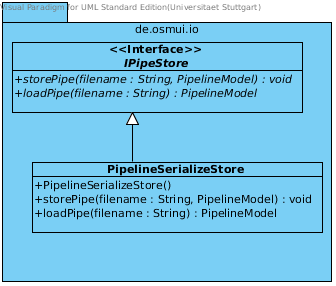
\includegraphics[width=8cm]{Schnittstelle_IPipeStore.png}
\end{center}
\subsubsection{Protokoll}
Laden: \\
Die Komponente bekommt einen Filename und lädt dann die Datei.
Speichern: \\
Die Komponente bekommt einen Filename und PipelineModel und speichert dann.
\subsubsection{Verhalten}
\subsubsection{Interne Realisierung}
\subsubsection{Realisierte Anforderungen}

\subsection{Komponente: ConfigurationsManager}
Die Komponente ConfigurationsManager übernimmt die Funktionalität der Konfiguration von OsmUi.
\subsubsection{Schnittstelle}
\begin{center}
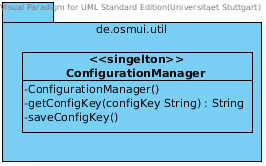
\includegraphics[width=7cm]{Schnittstelle_ConfigurationManager.png}
\end{center}
\subsubsection{Protokoll}
Die Komponente gibt auf Anfrage Informationen über die Konfiguration zurück.
\subsubsection{Verhalten}
\subsubsection{Interne Realisierung}
\subsubsection{Realisierte Anforderungen}


\subsection{Komponente: Application}
Die Application stellt das Hauptfenster bereit, in dem alle Oberflächenelemente enthalten sind.
Sie verkabelt die Eventhandler der anderen Komponenten und kümmert sich um die restliche Benutzerinteraktion wie zum Beispiel die Menüleiste oder die Kopierleiste.
\subsubsection{Schnittstelle}
Die Application hat keine externen Schnittstellen, abgesehen von ihrem Konstruktor
\subsubsection{Protokoll}
Laden: \\
Die Komponente bekommt einen Filename und lädt dann die Datei.
Speichern: \\
Die Komponente bekommt einen Filename und PipelineModel und speichert dann.
\subsubsection{Verhalten}
\subsubsection{Interne Realisierung}
Die Application nutzt das Singelton pattern um ihre Singularität innerhalb von OsmUi zu verdeutlichen und eventuell Zugriff durch die anderen Komponenten zu ermöglichen.
\subsubsection{Realisierte Anforderungen}
Zusammenführen der Komponenten


\subsection{Verbindungen}
\section{Externe Schnittstellen}
\subsection{Dauerhafte Datenspeicherung}
Die geplante Implementierung, sieht vor Pipelines aus/in bash- und bat-Scripten zu importieren/exportieren, Pipelines aus der Zwischenablage zu importieren und aus/in .smu Dateien Piplines zu Laden/Speichern. Außerdem soll die Programmkonfiguration in in das Heimat-/Konfigurationsverzeichnisses des Benutzers gespeichert werden. Diese Speicherung erfolgt in einem für Menschen lesbaren XML Format in eine .conf Datei.
\subsubsection{Datei/Datenbank: .smu}
In dieser Datei wird die Pipline. Um die Daten in/aus dieser Datei zu speichern/laden wir das Serialisierungsverfahren von Java benutzt 
\subsubsection{Datei/Datenbank: .conf}
Diese  Dateiformat dient dazu die Systemeinstellungen von Osmui zu speichern die geschieht im XML-Format. Zu den zu speichernden Informationen gehören der Osmosis-Pfad.
\subsubsection{Datei/Datenbank: .dat}
Dieses Dateiformat dient dazu ein Script bereitzustellen, mit dem der Benutzer den generierten Osmosis Aufruf unter Windows Systemen leicht ausführen kann. Dies wird dadurch realisiert, dass der Osmosispfad mit den zugehörigen Tasks und deren Parametern der ersten Zeile steht.
\subsubsection{Datei/Datenbank: .sh}
Dieses Dateiformat dient dazu ein Script bereitzustellen, mit dem der Benutzer den generierten Osmosis Aufruf unter Unix Systemen leicht ausführen kann. Dies wird dadurch realisiert, dass als Header \glqq \#!/bin/sh" geschrieben ist. In der darauf folgenden Zeile befindet sich der Osmosis-Pfad mit den zugehörigen Tasks und deren Parametern.
%\subsection{Externer Zugriff}

%\subsubsection{Schnittstelle: XYZ}

\appendix%

\section{Anhang}

\section{Literatur zum Entwurf}
\subsection{Entwurf}
\subsection{Entwurfsmuster}
\section{Versionshistorie}
\begin{itemize}
\item Version 1.0 8.12.2010 : Initialisierung
\item Version 1.1 9.12.2010 : Komponentennamen festgelegt
\item Version 1.2 10.12.2010 : Klassendiagramme für Komponenten hinzugefügt
\item Version 1.3 11.12.2010 : Komponentenbeschreibungen, Externe Schnittstellen hinzugefügt
\end{itemize}

\end{document}